% Chapter 3
\chapter{Insights} % Main c%----------------------------------------------------------------------------------------

\section{Identification of the research gap}

The advent of the IEC 61850 standard has significantly revolutionized the substation automation systems by facilitating interoperability and enhancing communication efficiency. Particularly, IEC 61850-9-2, which specifies the transmission of SV from MU to protection and control devices, has been pivotal in this transformation. Despite the substantial body of literature focusing on the implementation and benefits of IEC 61850-9-2, there remains a notable gap concerning the development of algorithms designed to optimize the selection of SVs in real-time protection scenarios involving multiple merging units.

\subsection{Existing Literature and Related Research}

A comprehensive literature review was conducted using databases such as IEEE Xplore, ScienceDirect, and Google Scholar. Keywords included "IEC 61850-9-2", "sampled values", "merging units", "protection relay", and "algorithm optimization". The search encompassed studies published from 2000 to 2023. The review revealed numerous studies addressing various aspects of IEC 61850-9-2, such as its implementation challenges, communication performance, and impact on substation automation.

For example,(~\cite{AbbReport2010}) explores the general benefits of IEC 61850-9-2 in improving the accuracy and speed of data transmission in substations. Similarly, (~\cite{baumgartner2024iec}) investigates the synchronization issues in SV transmission and proposes methods to mitigate these challenges. Additionally, (~\cite{chen2016performance})  examines the integration of IEC 61850-9-2 with other substation protocols to enhance system reliability.

\subsection{Identification of the Gap}

Despite these valuable contributions, none of the reviewed studies specifically address the development of an algorithm to select the optimal SV from multiple MUs for protection relays. This gap is critical, given the increasing complexity of modern substations where multiple MUs may collect data from the same current transformers (CTs), leading to potential conflicts and inefficiencies in data selection for protection purposes.

For instance, while (~\cite{IEC61850_SEL_9_2}) discusses the general principles of SV selection, it does not propose a concrete algorithmic approach to dynamically choose the best SV in real-time. Moreover, (~\cite{galkin2024microcomputer}) focuses on the latency and performance of SV transmission but does not consider the scenario of multiple MUs and the subsequent need for optimal SV selection.

\subsection{Importance of Addressing the Gap}

Addressing this gap is essential for several reasons. First, the ability to dynamically select the best SV from multiple MUs can significantly enhance the reliability and speed of protection relays, thereby improving overall substation safety and performance. Second, developing such an algorithm can provide a blueprint for future research and practical implementations, fostering further advancements in substation automation.

By focusing on the development of an algorithm that selects the optimal SV arriving before the protection relay, this research aims to fill a crucial void in the existing literature. This study will not only propose a novel solution to the identified problem but also provide empirical validation through simulations and real-world testing, thereby contributing valuable insights and practical tools to the field of substation automation and protection.

\subsection{Conclusion of the research gap}

In summary, while the IEC 61850-9-2 standard has been extensively studied, there remains a significant gap concerning the development of real-time algorithms for optimal SV selection from multiple MUs. This research aims to address this gap, providing a much-needed solution that enhances protection relay performance and overall substation reliability.

\section{Architecture of the Algorithm}

The algorithm involves receiving two measurements from the same measuring sensor (Current Transformers or Voltage Transformers), providing redundancy in the data acquisition required by the IED to process electrical protection algorithms. From a critical acquisition perspective, this approach is beneficial to address the scenario where one Merging Unit fails; the other Merging Unit can still send the data from that sensor. However, from the perspective of the IED, it needs to determine which of the two samples to use for running the protection algorithm to detect faults that may or may not occur based on the measurements received by the Merging Unit.

To address this issue, the proposed solution involves developing an algorithm that first monitors the SVs, classifying them, and then delivering only the sample that is most well-qualified to run the protection algorithms. The architecture of this solution is akin to a switch, where two or more SVs from the same current or voltage transformer arrive, and the switch allows only the path of the best-qualified sample, discarding the others. Consequently, two SVs may arrive, but the protection system will only consider one SVs with the best metric, Figure~\ref{fig:SLD_Diagram}~\footnote{\url{https://www.efacec.pt/en/wp-content/uploads/2022/08/CS491I2207A1_MCU-500.pdf}}, shown has a simple connection.

\begin{figure}[tbh]
	\centering
	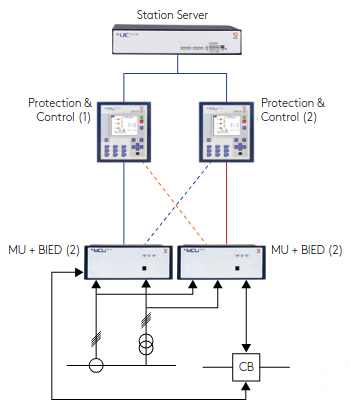
\includegraphics[width=0.77\textwidth, keepaspectratio]{ch3/assets/SLD_Diagram.png}
	\caption{Simple Single Line Diagram (SLD) of Electrical Substation with SV's. (Credits: Efacec Energia, Máquinas e Equipamentos Eléctricos, S.A.)}
	\label{fig:SLD_Diagram}
\end{figure}
\FloatBarrier
